\documentclass[11pt,a4paper]{article}
\usepackage[utf8]{inputenc}
\usepackage[T1]{fontenc}
\usepackage{ae}
\usepackage{mathtools}
\usepackage{amsfonts,amsmath,amssymb,amsthm}
\usepackage[libertine,cmintegrals,cmbraces,vvarbb]{newtxmath}
\usepackage[english]{babel}
\usepackage{cancel}
\usepackage{enumerate}
\usepackage[pdftex]{graphicx}
\usepackage{float}
\usepackage{caption}
\usepackage{subcaption}
\usepackage{listings}
\usepackage{fancyhdr}
\pagestyle{fancy}
\usepackage{fancybox}
\usepackage[dvipsnames]{xcolor}
\usepackage{tikz}
\usetikzlibrary{matrix,arrows,decorations.pathmorphing}
\usepackage{verbatim}
\usepackage{marvosym}
\usepackage{algorithm2e}
\usepackage{color}
\usepackage{bm}
\usepackage{todonotes}
\usepackage{listings}

\makeatletter
\newcommand\todoname{todo}
\newcommand\listtodoname{List of todos}
\makeatother

\setlength{\parindent}{0em}

\newcommand{\F}[0]{\mathbb{F}}
\newcommand{\N}[0]{\mathbb{N}}
\newcommand{\Z}[0]{\mathbb{Z}}
\newcommand{\Q}[0]{\mathbb{Q}}
\newcommand{\R}[0]{\mathbb{R}}
\newcommand{\C}[0]{\mathbb{C}}
\newcommand{\B}[0]{\mathbb{B}}
\newcommand{\im}[0]{\mathit{i}}
\newcommand{\uber}[2]{{{#1} \choose {#2}}}
\newcommand{\vect}[1]{\begin{pmatrix}#1\end{pmatrix}}
\newcommand{\norm}[1]{\left\lvert #1 \right\rvert}

\def\students{Willi Gierke, Arik Elimelech, Mehmed Halilovic, Leon Sixt}

\fancyhead[L]{SS 2017}
\fancyhead[C]{Maschinelles Lernen 2}
\fancyhead[R]{Assignment 08 -- \textbf{ESHG}}
\fancyfoot[L]{}
\fancyfoot[C]{\students}
\fancyfoot[R]{}


\title{Machine Learning 2 -- Group ESHG \\
        Assignment 09
}

\author{\students}
\date{\today}

\begin{document}
\maketitle

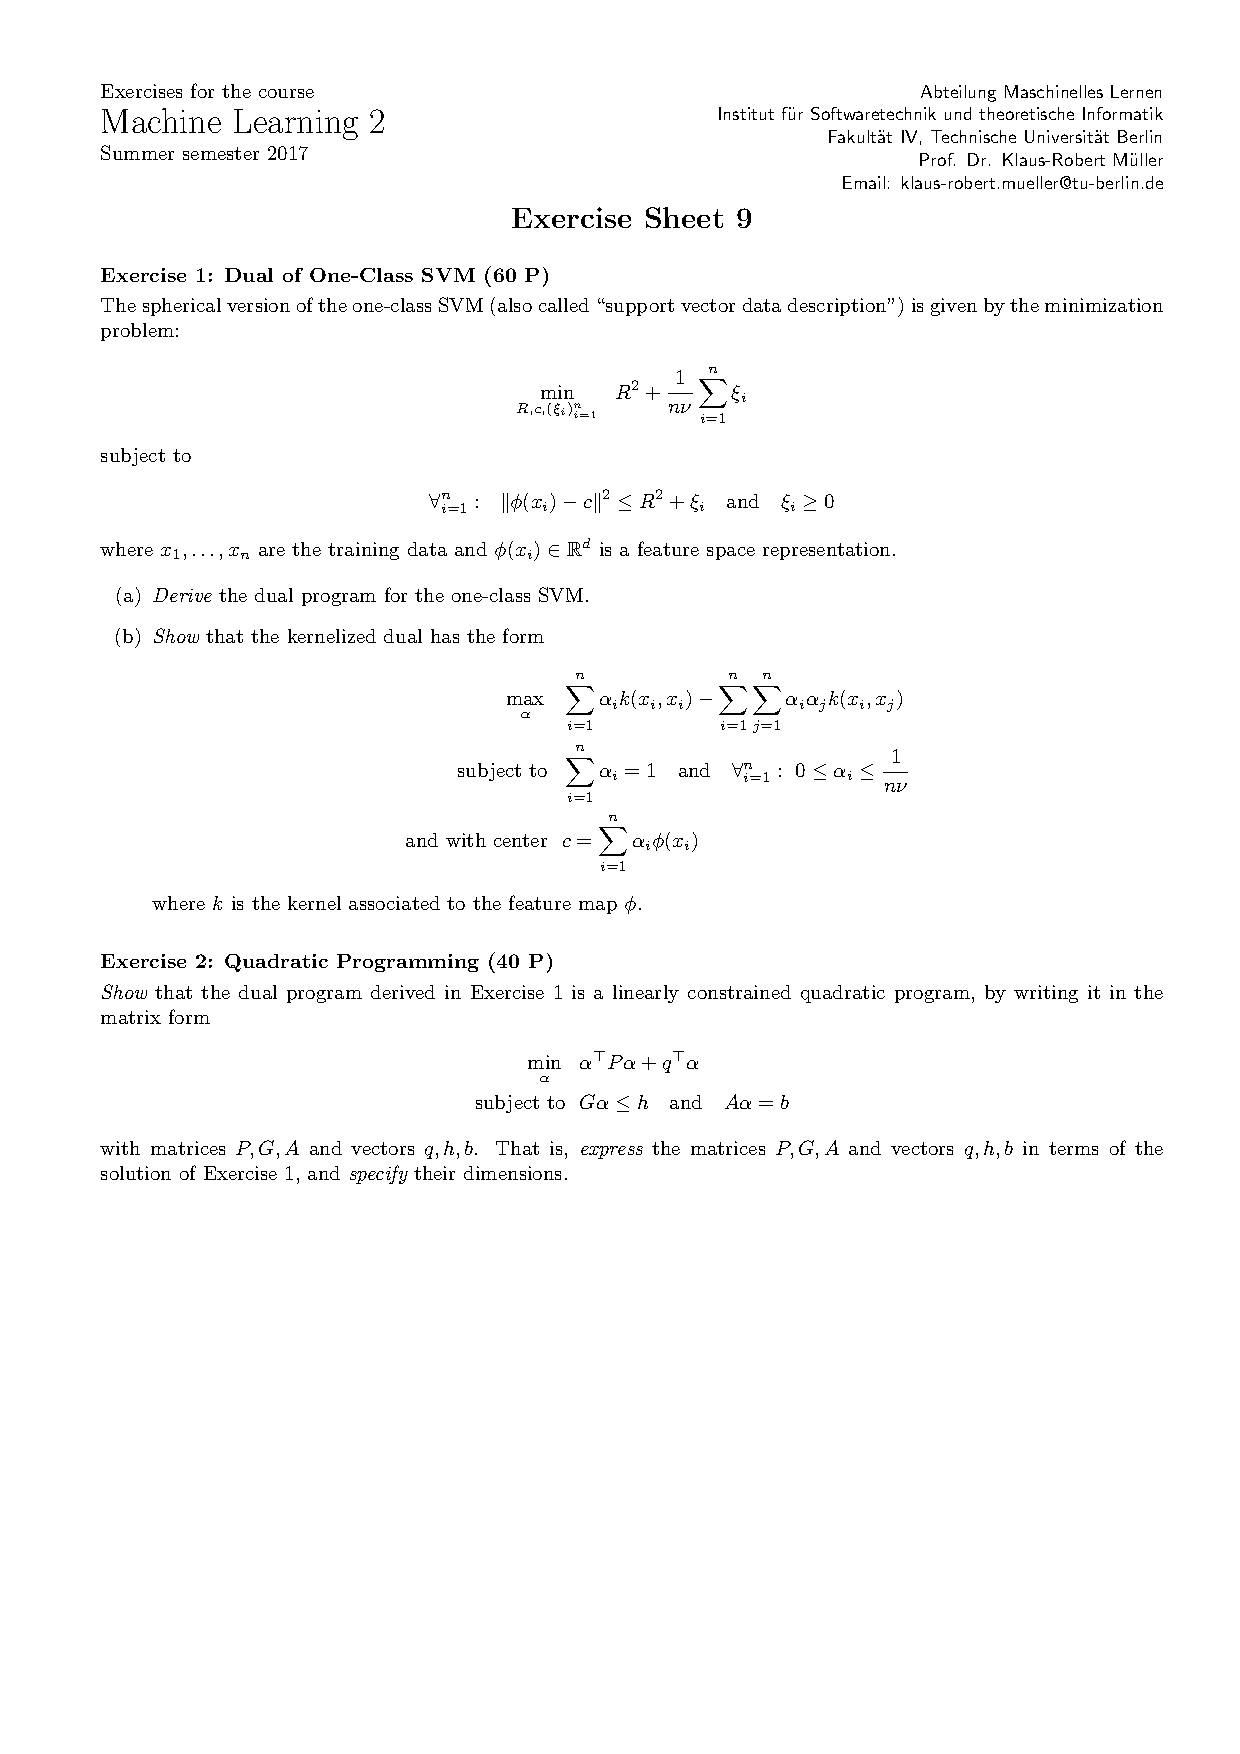
\includegraphics[clip, trim=0.5cm 2.5cm 0.5cm 4cm, width=0.90\textwidth]{sheet09.pdf}

\section*{Task 1}

\subsection*{a}
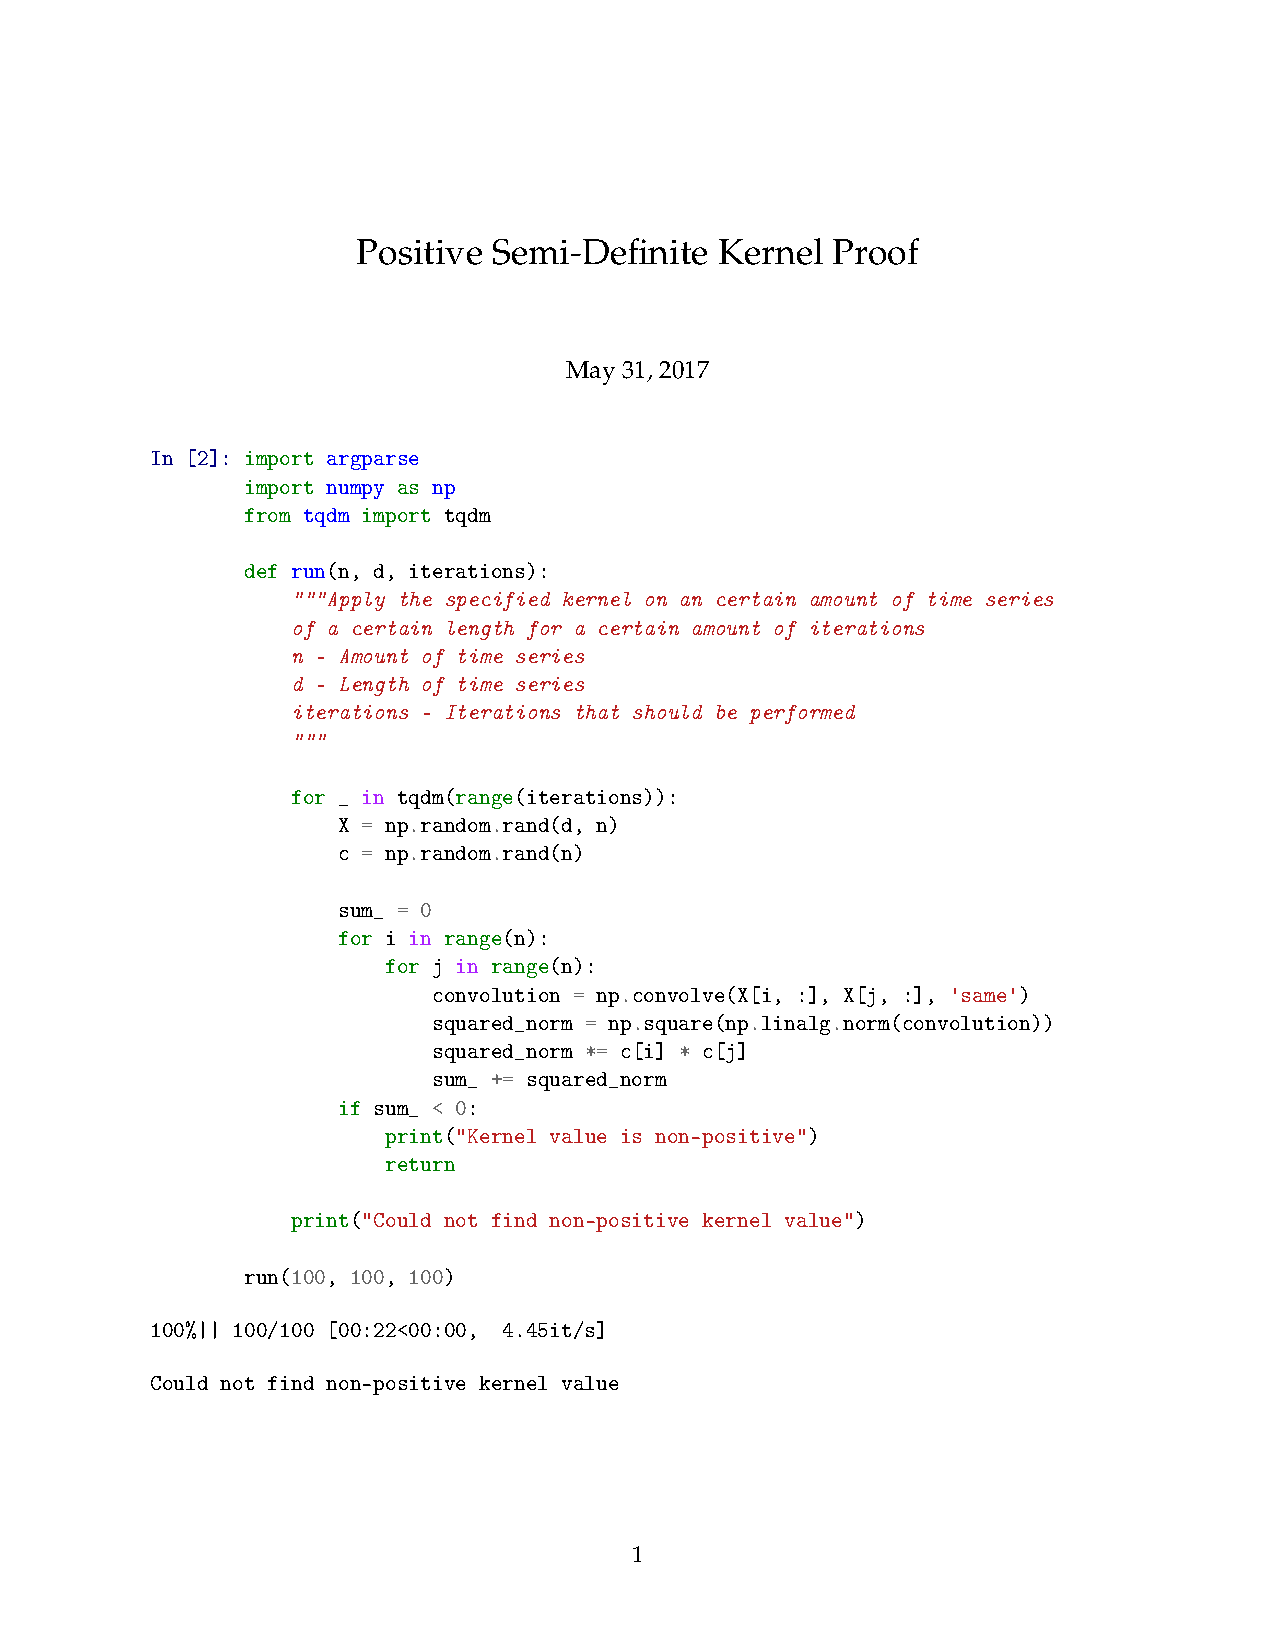
\includegraphics[clip, trim=0.5cm 2.5cm 0.5cm 4cm, width=0.90\textwidth]{KernelProof.pdf}

\subsection*{b}

The kernel is given by:

\begin{equation}
    k(x, y) = \lVert x * y \rVert ^ 2
\end{equation}

To be positive semi-definite, the kernel has to fulfill:

\begin{equation}
    \sum_{i=1}^n \sum_{j=1}^n c_i c_j k(x_i, x_j)
\end{equation}
for $n \in \N$, $\{x_1, \ldots, x_n\} \in \R^{d \times n} $ and $c \in \R^n$.
\\
\\
For the given kernel:
\begin{align}
    \sum_{i=1}^n \sum_{j=1}^n c_i c_j \lVert x_i * x_j \rVert ^ 2  \\
    = \sum_{i=1}^n \sum_{j=1}^n c_i c_j \sum_{t=0}^T (x_i * x_j)_t^2  \\
\end{align}

We can rewrite the convolution as fourier transformation.
Here, $\hat x_i $ denotes the fourier transform of $x_i$ and $F^{-1}$ the inverse
fourier transformation.
\begin{align}
    & \lVert x_i * x_j \rVert ^ 2 = \\
    &    = \Vert F^{-1}(\hat x_i \cdot  \hat x_j) \rVert ^ 2  \\
\end{align}

We assume that the feature space, ask for in the exercise, is connected to the
fourier transformation of x. However, the inverse fourier transform obstruct
us to separate the kernel into two feature maps.


\end{document}
